%%%%%%%%%%%%%%%%%%%%%%%%%%%%% Define Article %%%%%%%%%%%%%%%%%%%%%%%%%%%%%%%%%%
\documentclass{article}
%%%%%%%%%%%%%%%%%%%%%%%%%%%%%%%%%%%%%%%%%%%%%%%%%%%%%%%%%%%%%%%%%%%%%%%%%%%%%%%

%%%%%%%%%%%%%%%%%%%%%%%%%%%%% Using Packages %%%%%%%%%%%%%%%%%%%%%%%%%%%%%%%%%%
\usepackage{geometry}
\usepackage{graphicx}
\usepackage{amssymb}
\usepackage{amsmath}
\usepackage{amsthm}
\usepackage{empheq}
\usepackage{mdframed}
\usepackage{booktabs}
\usepackage{lipsum}
\usepackage{graphicx}
\usepackage{color}
\usepackage{psfrag}
\usepackage{pgfplots}
\usepackage{bm}
%%%%%%%%%%%%%%%%%%%%%%%%%%%%%%%%%%%%%%%%%%%%%%%%%%%%%%%%%%%%%%%%%%%%%%%%%%%%%%%

% Other Settings

%%%%%%%%%%%%%%%%%%%%%%%%%% Page Setting %%%%%%%%%%%%%%%%%%%%%%%%%%%%%%%%%%%%%%%
\geometry{a4paper}

%%%%%%%%%%%%%%%%%%%%%%%%%% Define some useful colors %%%%%%%%%%%%%%%%%%%%%%%%%%
\definecolor{ocre}{RGB}{243,102,25}
\definecolor{mygray}{RGB}{243,243,244}
\definecolor{deepGreen}{RGB}{26,111,0}
\definecolor{shallowGreen}{RGB}{235,255,255}
\definecolor{deepBlue}{RGB}{61,124,222}
\definecolor{shallowBlue}{RGB}{235,249,255}
%%%%%%%%%%%%%%%%%%%%%%%%%%%%%%%%%%%%%%%%%%%%%%%%%%%%%%%%%%%%%%%%%%%%%%%%%%%%%%%

%%%%%%%%%%%%%%%%%%%%%%%%%% Define an orangebox command %%%%%%%%%%%%%%%%%%%%%%%%
\newcommand\orangebox[1]{\fcolorbox{ocre}{mygray}{\hspace{1em}#1\hspace{1em}}}
%%%%%%%%%%%%%%%%%%%%%%%%%%%%%%%%%%%%%%%%%%%%%%%%%%%%%%%%%%%%%%%%%%%%%%%%%%%%%%%

%%%%%%%%%%%%%%%%%%%%%%%%%%%% English Environments %%%%%%%%%%%%%%%%%%%%%%%%%%%%%
\newtheoremstyle{mytheoremstyle}{3pt}{3pt}{\normalfont}{0cm}{\rmfamily\bfseries}{}{1em}{{\color{black}\thmname{#1}~\thmnumber{#2}}\thmnote{\,--\,#3}}
\newtheoremstyle{myproblemstyle}{3pt}{3pt}{\normalfont}{0cm}{\rmfamily\bfseries}{}{1em}{{\color{black}\thmname{#1}~\thmnumber{#2}}\thmnote{\,--\,#3}}
\theoremstyle{mytheoremstyle}
\newmdtheoremenv[linewidth=1pt,backgroundcolor=shallowGreen,linecolor=deepGreen,leftmargin=0pt,innerleftmargin=20pt,innerrightmargin=20pt,]{theorem}{Theorem}[section]
\theoremstyle{mytheoremstyle}
\newmdtheoremenv[linewidth=1pt,backgroundcolor=shallowBlue,linecolor=deepBlue,leftmargin=0pt,innerleftmargin=20pt,innerrightmargin=20pt,]{definition}{Definition}[section]
\theoremstyle{myproblemstyle}
\newmdtheoremenv[linecolor=black,leftmargin=0pt,innerleftmargin=10pt,innerrightmargin=10pt,]{problem}{Problem}[section]
%%%%%%%%%%%%%%%%%%%%%%%%%%%%%%%%%%%%%%%%%%%%%%%%%%%%%%%%%%%%%%%%%%%%%%%%%%%%%%%

%%%%%%%%%%%%%%%%%%%%%%%%%%%%%%% Plotting Settings %%%%%%%%%%%%%%%%%%%%%%%%%%%%%
\usepgfplotslibrary{colorbrewer}
\pgfplotsset{width=8cm,compat=1.9}
%%%%%%%%%%%%%%%%%%%%%%%%%%%%%%%%%%%%%%%%%%%%%%%%%%%%%%%%%%%%%%%%%%%%%%%%%%%%%%%

%%%%%%%%%%%%%%%%%%%%%%%%%%%%%%% Title & Author %%%%%%%%%%%%%%%%%%%%%%%%%%%%%%%%
\title{Derivative}
\author{Patrick Chen}
\date{Sept 18, 2024}
%%%%%%%%%%%%%%%%%%%%%%%%%%%%%%%%%%%%%%%%%%%%%%%%%%%%%%%%%%%%%%%%%%%%%%%%%%%%%%%

\begin{document}
    \maketitle
    \section*{The Derivative Function}
    \begin{align*}
        f'(x) =& \lim_{h\to 0} \frac{f(x+h)-f(x)}{h} \\
        f:&\ \mathbb{R} \mapsto \mathbb{R} \\
        f':&\ \mathbb{R} \mapsto \mathbb{R} \\
        f':&\ x \mapsto \text{ the slope of the function } f
    \end{align*}

    \begin{align*}
        f(x) = 2x^2
    \end{align*}

    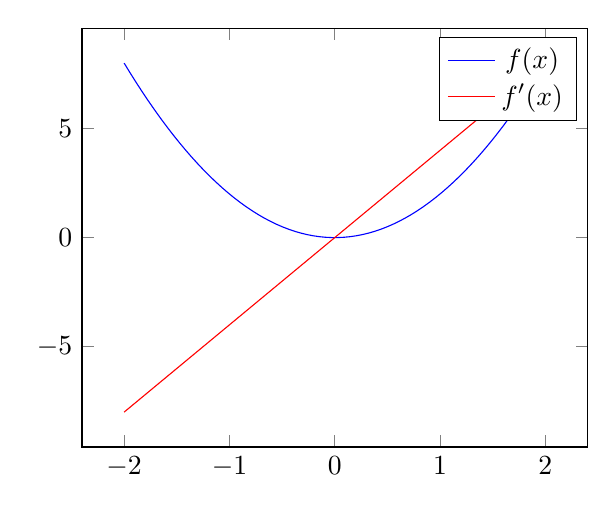
\begin{tikzpicture}
        \begin{axis}
            \addplot[
                domain=-2:2,
                samples=70,
                color=blue,
                ]
                {2*x*x};
            \addlegendentry{$f(x)$}
            \addplot [
                domain=-2:2,
                samples=70,
                color=red,
                ]
                {4*x};
            \addlegendentry{$f'(x)$}
        \end{axis}
    \end{tikzpicture}

    \begin{align*}
        f'(x)=y'= \frac{df}{dx} = \frac{dy}{dx} = \frac{d}{dx} f(x)
    \end{align*}
    A function $f$ is differentiable at $a$ if $f'(a)$ exists (and is finite).
    $f$ is differentiable on $(a,b)$ if $f$ is differentiable at every point in
    $(a,b)$.

    \section*{Example}
    \begin{align*}
        f(x) = |x-4|
    \end{align*}

    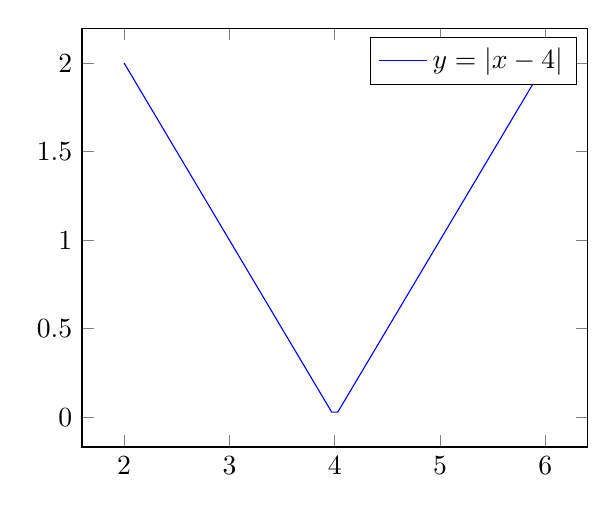
\begin{tikzpicture}
         \begin{axis}
             \addplot [
                domain=2:6,
                samples=70,
                color=blue,
                ]
                {abs(x-4)};
             \addlegendentry{$ y=|x-4|$}
         \end{axis}
    \end{tikzpicture}

    \begin{align*}
        |x-4| &= \begin{cases}
            x-4, & x-4\ge 0\\
            -(x-4) & x-4< 0
        \end{cases} \\
        f'(x) &= \begin{cases}
            1, & x>4 \\
            -1 & x<4 \\
            \text{undefined} & x=4
        \end{cases}
    \end{align*}

    $f'(0)$ is undefined because the left and right limits are not equal.
    \begin{align*}
        &\lim_{h\to 0^+} \frac{f(4+h)-f(4)}{h} \\
        =& \lim_{h\to 0^+} \frac{|h|}{h} \\
        &\text{$|h|$ and $h$ are positive} \\
        =& 1
    \end{align*}
    \begin{align*}
        &\lim_{h\to 0^-} \frac{f(4+h)-f(4)}{h} \\
        =& \lim_{h\to 0^-} \frac{|h|}{h} \\
        &\text{$|h|$ is positive but $h$ is negative} \\
        =& -1
    \end{align*}

    \begin{theorem}
        If f is differentiable at a, then f is continuous at a.
    \end{theorem}
    We saw this in the absolute value example. $|x-4|$ is continuous
    but not differentiable at point (4, 0).

    There are many ways a function cannot be differentiable.
    \begin{enumerate}
        \item Cusp \\
        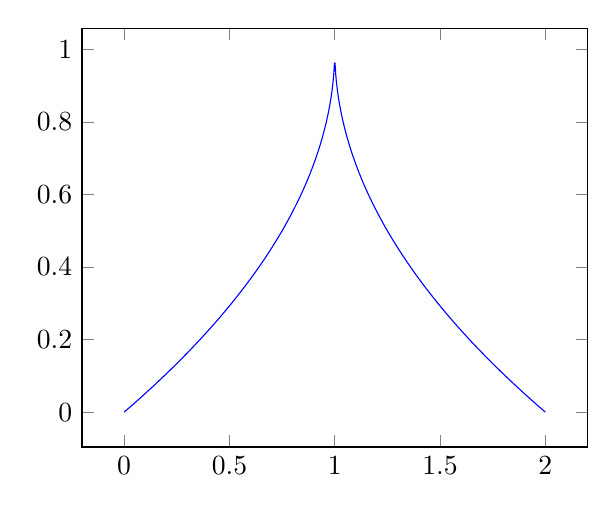
\begin{tikzpicture}
             \begin{axis}
                 \addplot [
                    domain=0:2,
                    samples=700,
                    color=blue,
                    ]
                    {-(sqrt(abs(x-1)))+1};
             \end{axis}
        \end{tikzpicture}

        \item Discontinuous and therefore not differentiable \\
        \begin{tikzpicture}
             \begin{axis}
                 \addplot [
                    domain=1:2,
                    samples=700,
                    color=blue,
                    ]
                    {x+2};
                 \addplot [
                    domain=0:1,
                    samples=700,
                    color=blue,
                    ]
                    {x};
             \end{axis}
        \end{tikzpicture}

        \item Infinite slope \\
        \begin{tikzpicture}
             \begin{axis}
                 \addplot [
                    domain=-1:1,
                    samples=700,
                    color=blue,
                    ]
                    {sign(x)*(abs(x))^(1/3)};
             \end{axis}
        \end{tikzpicture}
    \end{enumerate}

    \subsection*{Higher Derivatives}
    The derivative of the derivative of a function is called the second
    derivative of the function.
    \begin{align*}
        \frac{d}{dx} \frac{dy}{dx} = \frac{d^2y}{dx^2}
    \end{align*}
    \begin{align*}
        \frac{d}{dx} \frac{d}{dx} \dots \frac{d}{dx} \frac{dy}{dx}
        = \frac{d^ny}{dx^n}
    \end{align*}

    \section*{Derivative Rules}
    \subsection*{Constant Multiple, Addition, and Subtraction}
    \begin{align*}
        \frac{d}{dx} (cf(x)) &= c \frac{d}{dx} (f(x)) \\
        \frac{d}{dx} (f(x)+g(x)) &= \frac{d}{dx} (f(x)) + \frac{d}{dx} (g(x)) \\
        \frac{d}{dx} (f(x)-g(x)) &= \frac{d}{dx} (f(x)) - \frac{d}{dx} (g(x))
    \end{align*}

    \subsection*{Product and Quotient rules}
    When two functions are multiplied together (product rule):
    \begin{align*}
        \frac{d}{dx} (f(x)g(x)) &= f(x) \frac{d}{dx} (g(x)) + \frac{d}{dx} (f(x)) g(x) \\
        (fg)' &= f'g + fg'
    \end{align*}
    When one function is divided by another function (quotient rule):
    \begin{align*}
        \frac{d}{dx} (\frac{f(x)}{g(x)}) &= \frac{ \frac{d}{dx} (f(x)) g(x) - f(x) \frac{d}{dx} (g(x))}{g(x)^2} \\
        (\frac{f}{g})' &= \frac{f'g - fg'}{g^2}
    \end{align*}

    \subsection*{Chain rule}
    For a function $g$ that is differentiable at $x$ and a function $f$ that is
    differentiable at $f(x)$, the derivative of $f\circ g$ can be found using
    the chain rule.
    \begin{align*}
        y  &= f(g(x)) \\
        y' &= f'(g(x)) \cdot g'(x)
    \end{align*}

    Example:
    let $y = \sqrt{x^2+1}$
    \begin{align*}
        g(x) = x^2+1 &\Rightarrow g'(x)=2x \\
        f(x) = \sqrt{x} &\Rightarrow f'(x)= \frac{1}{2\sqrt{x}} \\
        y' = \frac{1}{2\sqrt{x^2+1}} 2x &= \frac{x}{\sqrt{x^2+1}}
    \end{align*}

    \subsection*{Implicit Differentiation}
    Implicit differentiation is the process of treating a $y$ like the function
    $f(x)$. This can be useful when it is difficult or impossible to isolate for
    y in a equation. The derivative of a curve can be found by using implicit
    differentiation then solving for $y'$.

    Example:
    \begin{align*}
        x^3+y^3&=6xy \\
               &\Downarrow \\
        x^3+f(x)^3 &= 6xf(x)
    \end{align*}

    \begin{align*}
        (y^3)' &= (f(x)^3)' \\
        &= 3f(x) \cdot f'(x) \\
        &= 3y \cdot y'
    \end{align*}

    \begin{align*}
        x^3+y^3                 &= 6xy \\
        3x^2 + 3y^2y'           &= 6(xy'+1y) \\
        3x^2+3y^2y'             &= 6xy'+6y \\
        3x^2-6y                 &= 6xy'-3y^2y' \\
        3x^2-6y                 &= (6x-3y^2)y' \\
        \frac{3x^2-6y}{6x-3y^2} &= y'
    \end{align*}

    This means the slope at the point $(x,y)$ is $\frac{3x^2-6y}{6x-3y^2}$

    \subsection*{Inverse Functions}
    If $f$ is a differentiable one-to-one function, the derivative of the
    inverse function can be found with the following formula.
    \begin{align*}
        (f^{-1})' = \frac{1}{f'(f(x))}
    \end{align*}
    Proof:
    \begin{align*}
        y &= f^{-1}(x) \\
        f(y) &= f(f^{-1}(x)) \\
        f(y) &= x \\
        f'(y)y' &= 1 & \text{implicit differentiation} \\
        y' &= \frac{1}{f'(y)} \\
        y' &= \frac{1}{f'(f(x))} & \text{substitute $y$} \\
    \end{align*}



    \section*{Derivatives of functions}
    \subsection*{Polynomial}
    The constant function:
    \begin{align*}
        f(x) = c \\
        \frac{d}{dx} (c) = 0
    \end{align*}
    \begin{align*}
        &\lim_{h\to 0} \frac{f(x+h)-f(x)}{h} \\
        =&\lim_{h\to 0} \frac{c-c}{h} \\
        =&\lim_{h\to 0} \frac{0}{h} \\
        =& 0
    \end{align*}
    \begin{tikzpicture}
        \begin{axis} [ymin=1, ymax=3]
             \addplot [
                domain=-1:1,
                samples=70,
                color=blue,
                ]
                {2};
         \end{axis}
    \end{tikzpicture}

    Linear (degree one) function:
    \begin{align*}
        f(x)=x \\
        \frac{d}{dx} (x) = 1
    \end{align*}
    \begin{tikzpicture}
         \begin{axis}
             \addplot [
                domain=-1:1,
                samples=70,
                color=blue,
                ]
                {x};
         \end{axis}
    \end{tikzpicture}

    Quadratic:
    \begin{align*}
        f(x)=x^2 \\
        \frac{d}{dx} (x^2) = 2x
    \end{align*}
    \begin{align*}
        &\lim_{h\to 0} \frac{(x+h)^2-x^2}{h} \\
        =&\lim_{h\to 0} \frac{x^2+2xh+h^2-x^2}{h} \\
        =&\lim_{h\to 0} \frac{2xh+h^2}{h} \\
        =&\lim_{h\to 0} 2x+h \\
        =&2x
    \end{align*}
    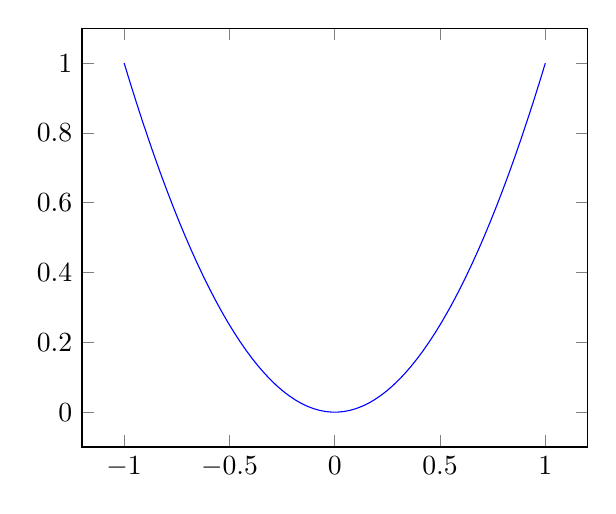
\begin{tikzpicture}
         \begin{axis}
             \addplot [
                domain=-1:1,
                samples=70,
                color=blue,
                ]
                {x^2};
         \end{axis}
    \end{tikzpicture}

    General:
    \begin{align*}
        f(x) &= x^n \\
        \frac{d}{dx} (x^n) &= nx^{n-1}
    \end{align*}

    \subsection*{Exponential}
    \begin{align*}
        \lim_{h\to 0} \frac{f(x+h)-f(x)}{h} \\
        \lim_{h\to 0} \frac{e^(x+h) - e^x}{h} \\
        \lim_{h\to 0} \frac{e^x e^h - e^x}{h} \\
        \lim_{h\to 0} \frac{e^x (e^h - 1)}{h} \\
        e^x \lim_{h\to 0} \frac{e^h - 1}{h} \\
    \end{align*}
    \begin{align*}
        \lim_{h\to 0} \frac{e^h - 1}{h} = 1
    \end{align*}

    The derivative of $e^x$ is itself.
    \begin{align*}
        \frac{d}{dx} e^x = e^x
    \end{align*}

    For an exponent with a different base, convert to base $e$ using logarithm
    rules.
    \begin{align*}
        a^x = e^{\ln (a^x)} = e^{x \ln(a)} \\
        (a^x)' = e^{x\ln(a)}\ln(a) = a^x \cdot \ln(a)
    \end{align*}

    \subsection*{Logarithm}

    \begin{align*}
        \frac{d}{dx} \ln x = \frac{1}{x}
    \end{align*}

    \begin{align*}
        y              &= \log_a x \\
        a^y            &= x \\
        (\ln a) a^y y' &= 1 \\
        y'             &= \frac{1}{(a^y)\ln a} \\
        y'             &= \frac{1}{x\ln a} \\
    \end{align*}

    \subsection*{Trigonometric Functions}
    \begin{align*}
        \frac{d}{dx} \sin(x) &= \cos(x) \\
        \frac{d}{dx} \cos(x) &= -\sin(x) \\
        \frac{d}{dx} \tan(x) &= \sec^2(x) \\
        \frac{d}{dx} \csc(x) &=  -\csc(x)\cot(x) \\
        \frac{d}{dx} \sec(x) &=  \sec(x)\tan(x) \\
        \frac{d}{dx} \cot(x) &=  -\csc^2(x)
    \end{align*}

    \begin{align*}
        &\lim_{h\to 0} \frac{\sin(x+h) - \sin(x)}{h} \\
        =&\lim_{h\to 0} \frac{\sin(x)\cos(h)+\cos(x)\sin(h)- \sin(x)}{h} \\
        =&\lim_{h\to 0} \frac{\sin(x)\cos(h)-\sin(x)}{h}
            + \lim_{h\to 0} \frac{\cos(x)\sin(h)}{h} \\
        =&\sin(x)\lim_{h\to 0} \frac{(\cos(h)-1)}{h}
            + \cos(x)\lim_{h\to 0} \frac{\sin(h)}{h} \\
        =&\sin(x)(0) + \cos(x)(1) \\
        =&\cos(x) \\
    \end{align*}

    \begin{align*}
        \lim_{\theta\to 0} \frac{\cos\theta-1}{\theta} = 1 &&
        \lim_{\theta\to 0} \frac{\sin\theta}{\theta} = 1
    \end{align*}

    \subsection*{Inverse Trigonometric Function}
    \begin{align*}
        \frac{d}{dx} \sin^{-1}(x) &= \frac{1}{\sqrt{1-x^2}} \\
        \frac{d}{dx} \cos^{-1}(x) &= -\frac{1}{\sqrt{1-x^2}} \\
        \frac{d}{dx} \tan^{-1}(x) &= \frac{1}{1+x^2} \\
        \frac{d}{dx} \sec^{-1}(x) &= \frac{1}{|x|\sqrt{x^2-1}} \\
        \frac{d}{dx} \csc^{-1}(x) &= - \frac{1}{|x|\sqrt{x^2-1}} \\
        \frac{d}{dx} \cot^{-1}(x) &= -\frac{1}{1+x^2}
    \end{align*}

\end{document}
